\documentclass[xcolor=x11names,compress]{beamer}
%%%%%%%%%%%%%%%%%%%%%%%%%%%%%%%%%%%%%%%%%%%%%%%%%%
\usepackage{graphicx}
\usepackage{tikz}
\usepackage[utf8]{inputenc}
\usepackage[T1]{fontenc}
\usepackage[francais]{babel}
\usetikzlibrary{decorations.fractals}
%%%%%%%%%%%%%%%%%%%%%%%%%%%%%%%%%%%%%%%%%%%%%%%%%%

%%%%%%%%%%%%%%%%%%%%%%%%%%%%%%%%%%%%%%%%%%%%%%%%%%
\useoutertheme[subsection=false,shadow]{miniframes}
\useinnertheme{default}
\usefonttheme{serif}
\usepackage{palatino}


\setbeamerfont{title like}{shape=\scshape}
\setbeamerfont{frametitle}{shape=\scshape}

\setbeamercolor*{lower separation line head}{bg=DeepSkyBlue4}
\setbeamercolor*{normal text}{fg=black,bg=white}
\setbeamercolor*{alerted text}{fg=red}
\setbeamercolor*{example text}{fg=black}
\setbeamercolor*{structure}{fg=black}
 
\setbeamercolor*{palette tertiary}{fg=black,bg=black!10}
\setbeamercolor*{palette quaternary}{fg=black,bg=black!10}

\renewcommand{\(}{\begin{columns}}
\renewcommand{\)}{\end{columns}}
\newcommand{\<}[1]{\begin{column}{#1}}
\renewcommand{\>}{\end{column}}
%%%%%%%%%%%%%%%%%%%%%%%%%%%%%%%%%%%%%%%%%%%%%%%%%%

\begin{document}


%%%%%%%%%%%%%%%%%%%%%%%%%%%%%%%%%%%%%%%%%%%%%%%%%%
\section{\scshape Introduction}
\begin{frame}{}
    \title{Blender}
    \author{
    	Aurélie Murcia \& Julien Roussé\\
	    {\it Université de Montpellier}\\
        }
    \date{
	    \begin{tikzpicture}
    		\draw[DeepSkyBlue4] decorate{ (0,0) -- (3,0) }; 
	    \end{tikzpicture}  
	\\
	\vspace{1cm}
	{2016 - 2017}
}
    \titlepage
\end{frame}

%%%%%%%%%%%%%%%%%%%%%%%%%%%%%%%%%%%%%%%%%%%%%%%%%%
\begin{frame}{Table des matières}
    \tableofcontents
\end{frame}


%%%%%%%%%%%%%%%%%%%%%%%%%%%%%%%%%%%%%%%%%%%%%%%%%%
\begin{frame}{Introduction}
    
\includegraphics[scale=0.2]{blogo} \textit{ Logo de Blender}
    \vspace{0.5cm}
    \begin{itemize}
        \item Logiciel de modélisation, d'animation et de rendu 3D
    \item Créé en 1995
    \item Le nom \textit{Blender} est une référence à une musique du groupe Yello
    \item Il présente l'avantage d'être un logiciel gratuit, libre et Open Source (depuis 2002)
    \item Blender est multiplate-forme : présent sur GNU, Linux, Windows, Mac, Solaris, ...
    \end{itemize}
\end{frame}

%%%%%%%%%%%%%%%%%%%%%%%%%%%%%%%%%%%%%%%%%%%%%%%%%%
\section{\scshape Présentation des outils de base}
\begin{frame}[c]{}
    \centering
    \huge
    \textbf{Présentation des outils de base}
\end{frame}

%%%%%%%%%%%%%%%%%%%%%%%%%%%%%%%%%%%%%%%%%%%%%%%%%%
\subsection{L'interface}
\begin{frame}[fragile, allowframebreaks]{L'interface}
    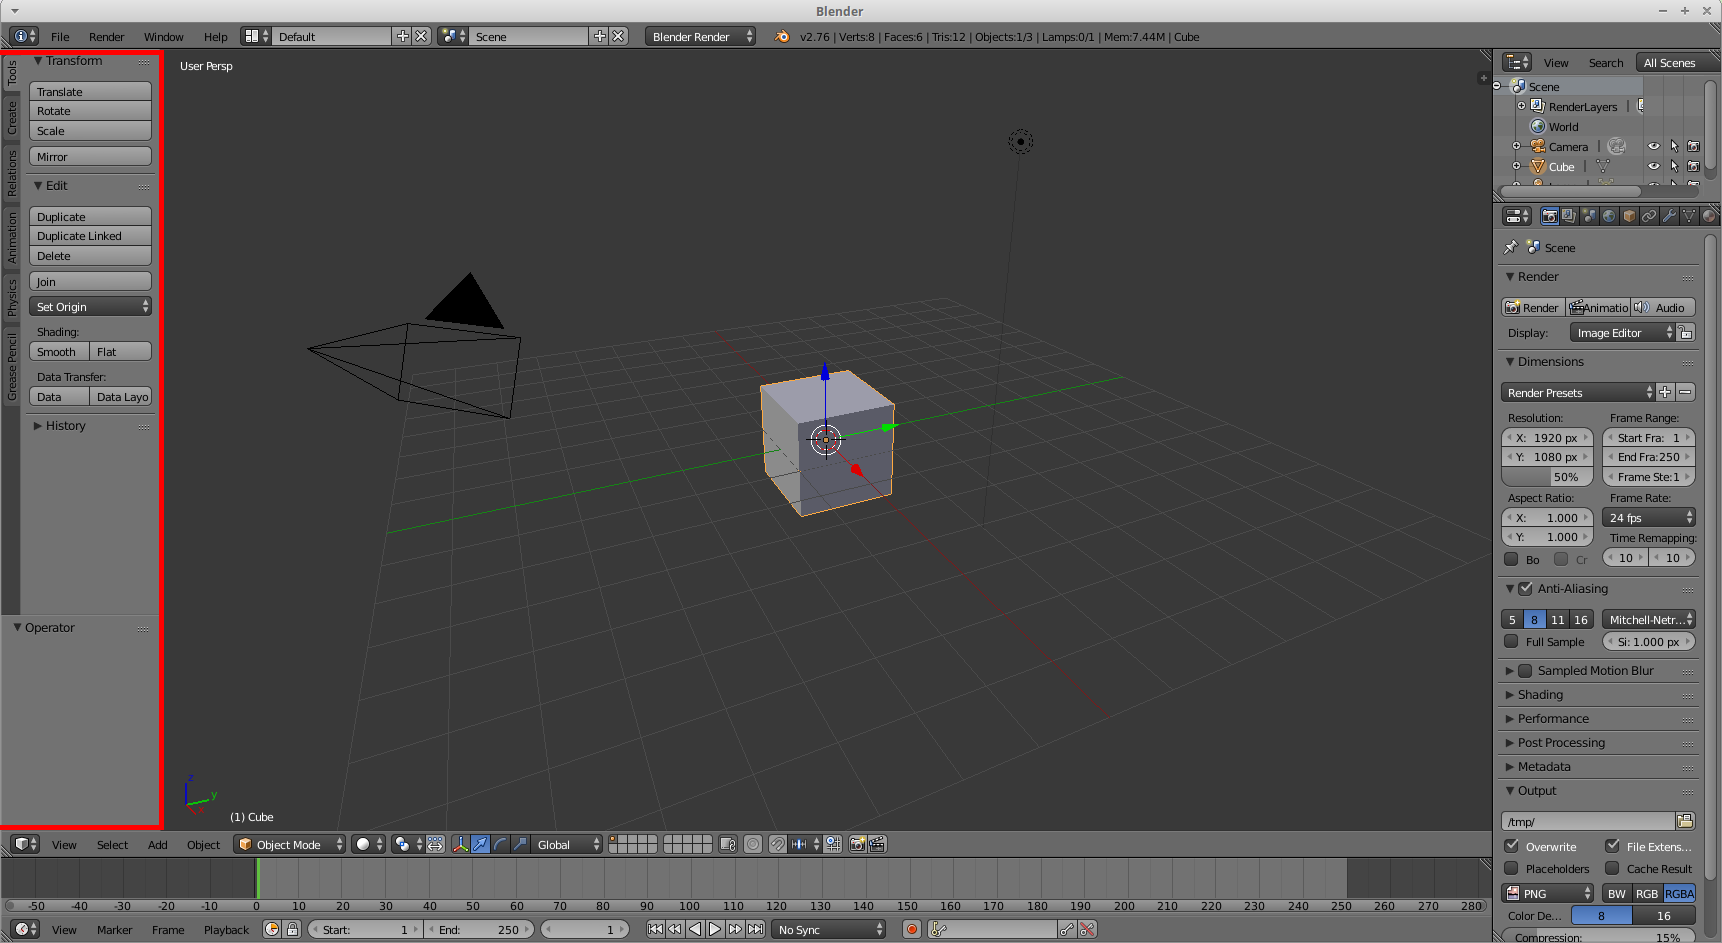
\includegraphics[scale=0.24]{menu_mesh}
    \vspace{1cm} 
    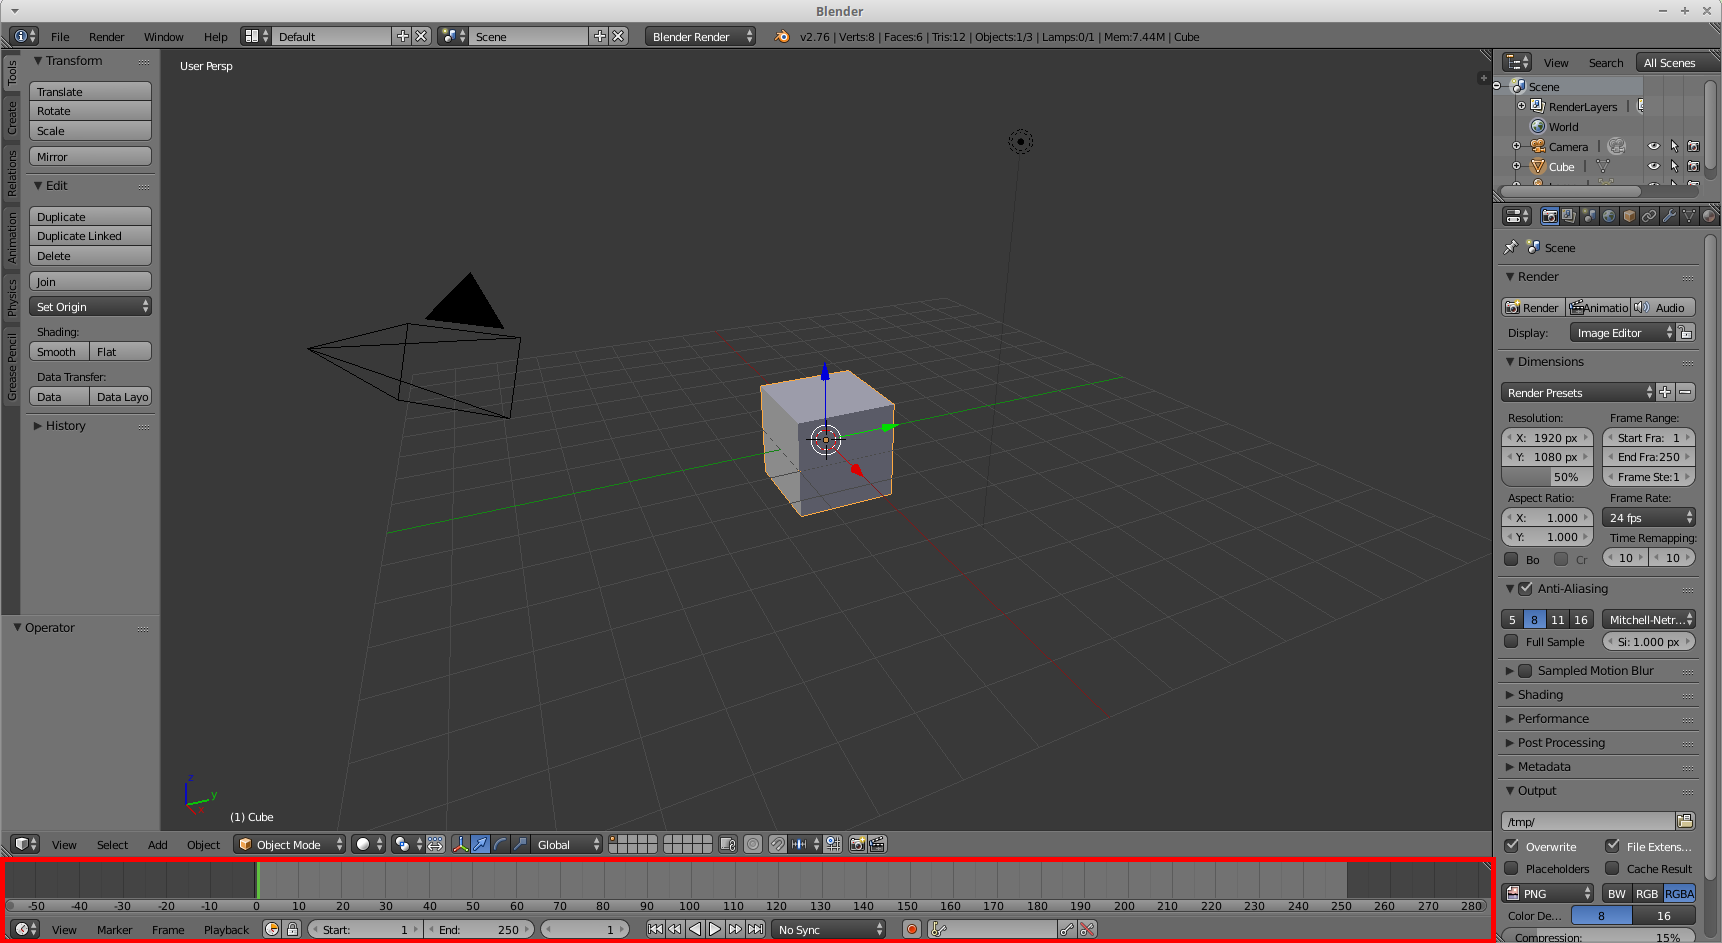
\includegraphics[scale=0.24]{menu_temps}
    \vspace{1cm}
    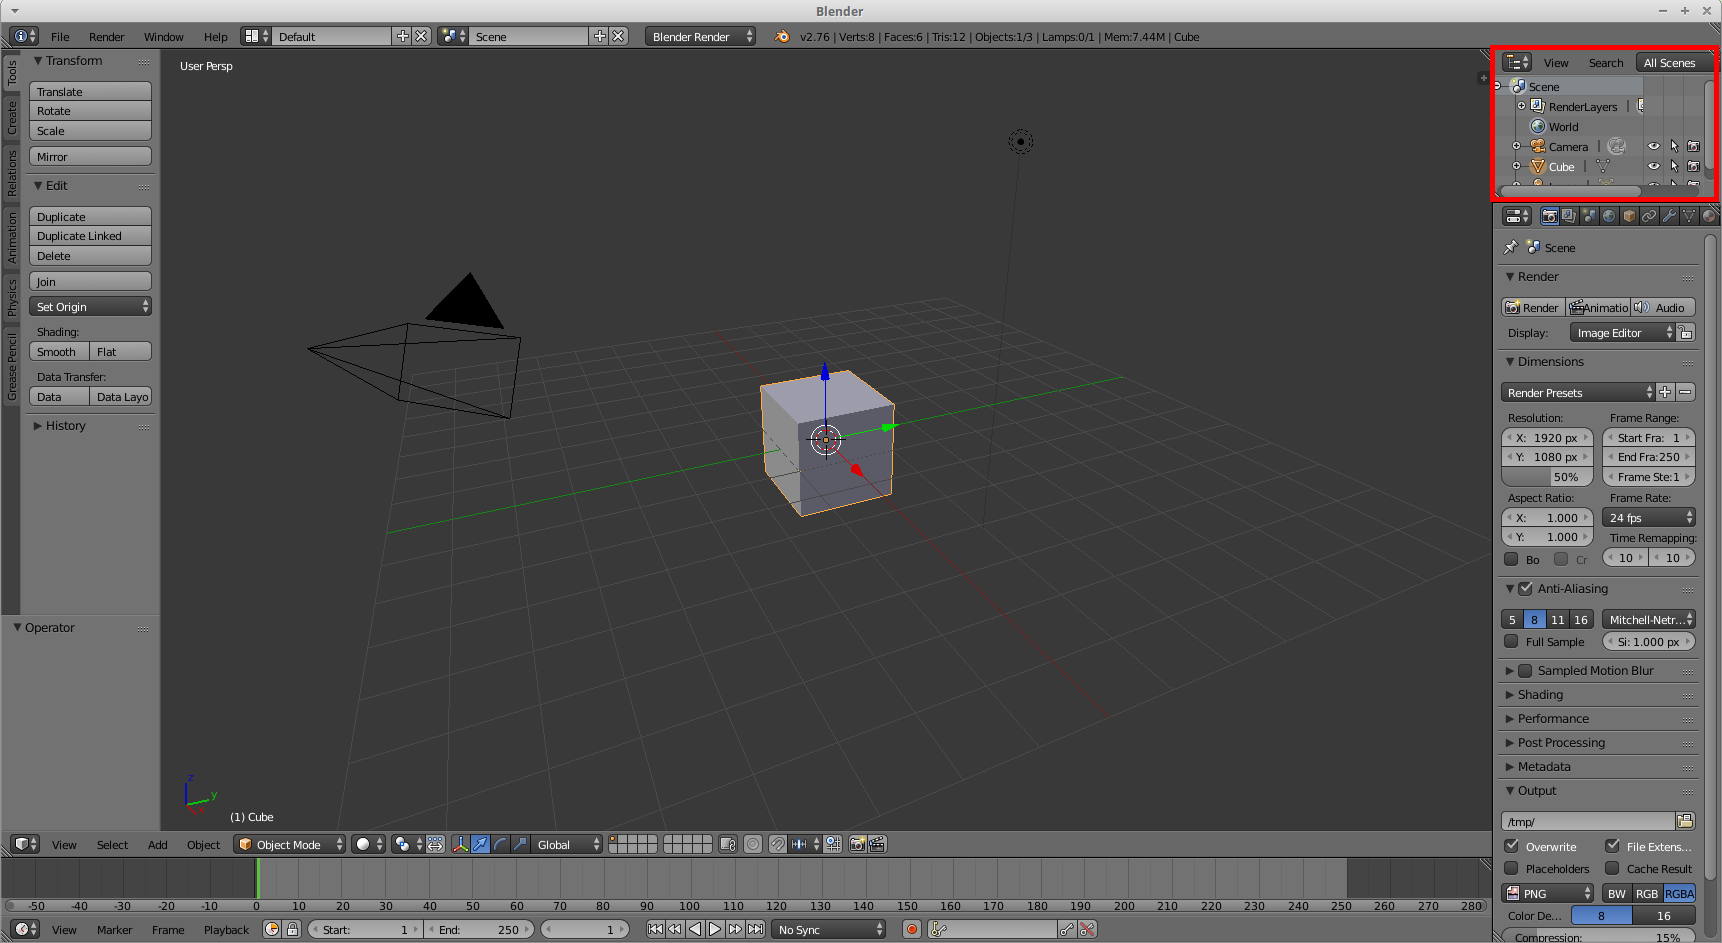
\includegraphics[scale=0.24]{tablematiere}
    \vspace{1cm}
    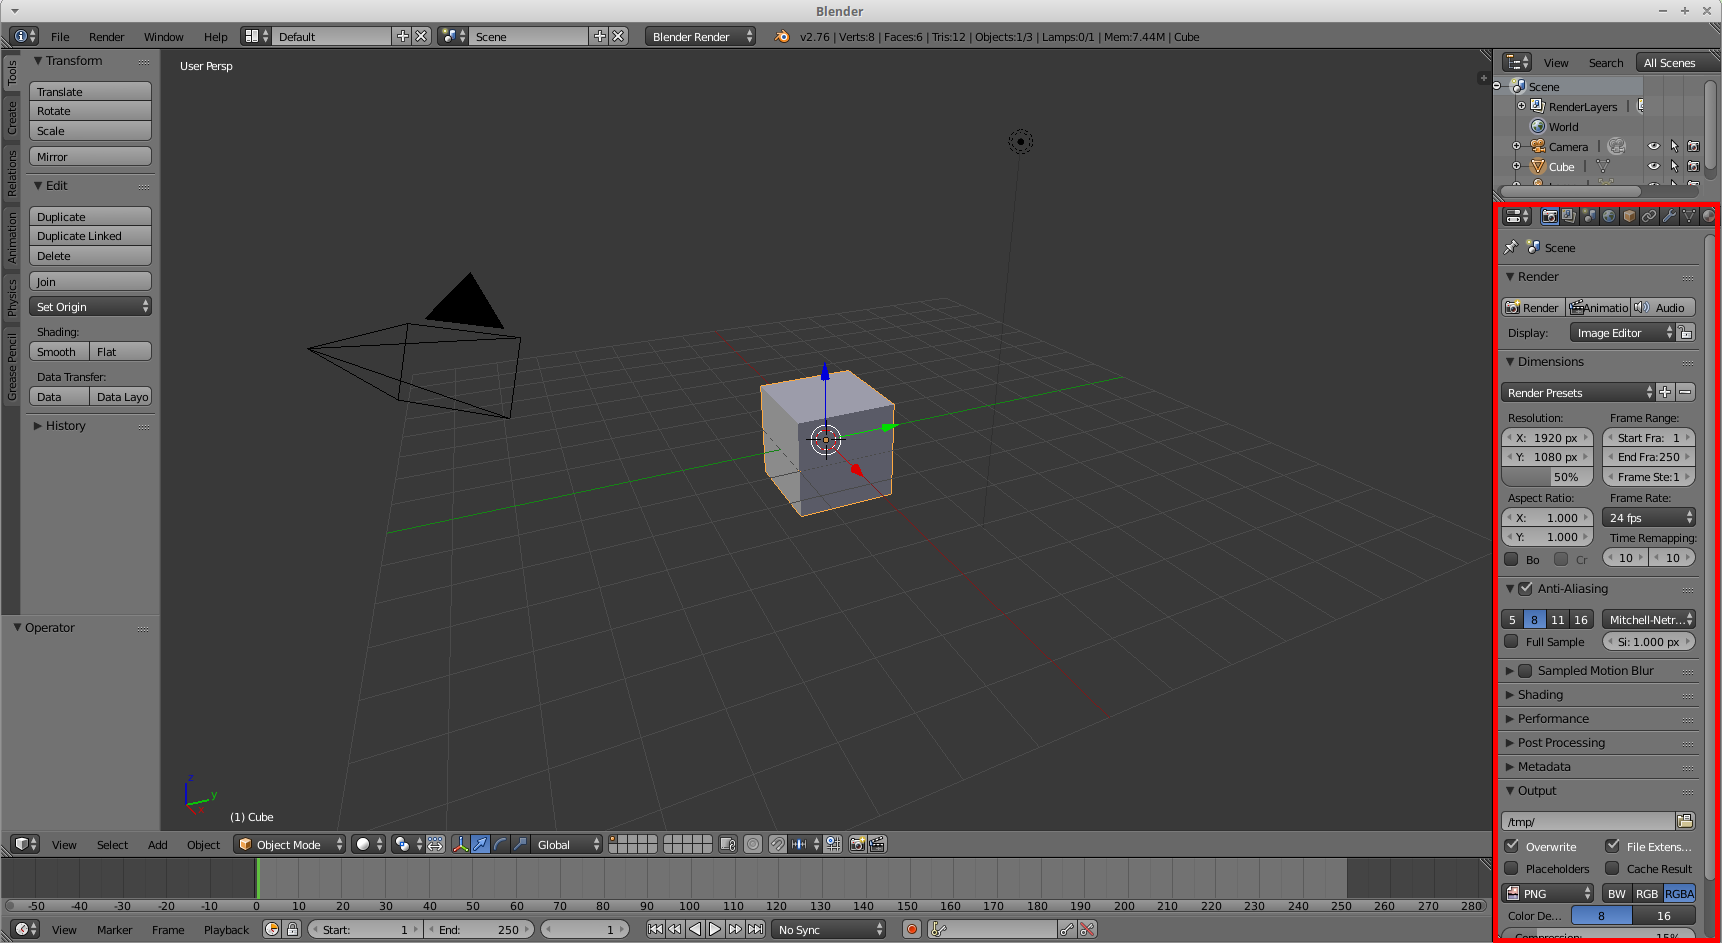
\includegraphics[scale=0.24]{menu_proprietes}
\end{frame}

%%%%%%%%%%%%%%%%%%%%%%%%%%%%%%%%%%%%%%%%%%%%%%%%%%
\subsection{Les meshes}
    \begin{frame}[fragile, allowframebreaks]{Les meshes}
        \begin{itemize}
        \item Mesh signifie maille
        \item Un mesh est un objet constitué de sommets, de faces et d'arêtes, qui sert de modèle de base aux créations plus complexes
        \item \textit{Présentation des meshes}
    \end{itemize}
    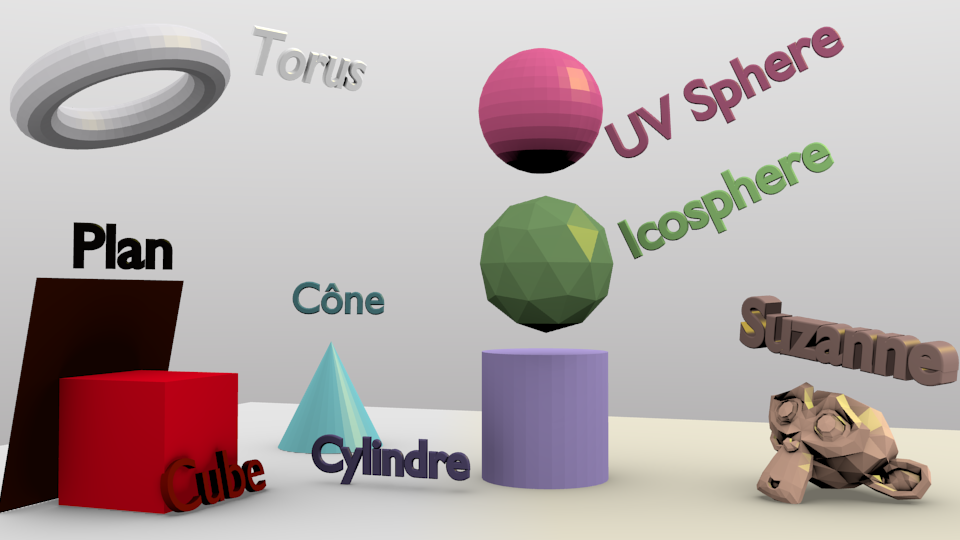
\includegraphics[scale=0.30]{meshrappel}
    \begin{flushright}
        \textit{Un petit récapitulatif des meshes}
    \end{flushright}
\end{frame}

%%%%%%%%%%%%%%%%%%%%%%%%%%%%%%%%%%%%%%%%%%%%%%%%%%
\subsection{La caméra}
\begin{frame}{La caméra}
 \centering 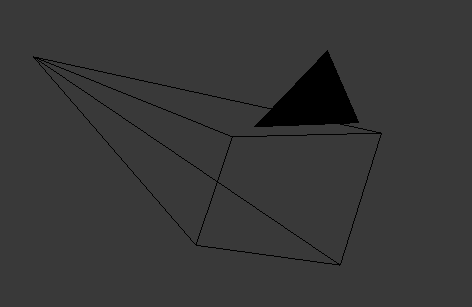
\includegraphics[scale=0.29]{camera}
    \begin{itemize}
        \item Détermine le rendu final
        \item Si la scène ne comporte aucune caméra, tenter un rendu produira une erreur
\end{itemize}
\end{frame}

%%%%%%%%%%%%%%%%%%%%%%%%%%%%%%%%%%%%%%%%%%%%%%%%%%
\subsection{La lampe}
\begin{frame}[fragile, allowframebreaks]{La lampe}
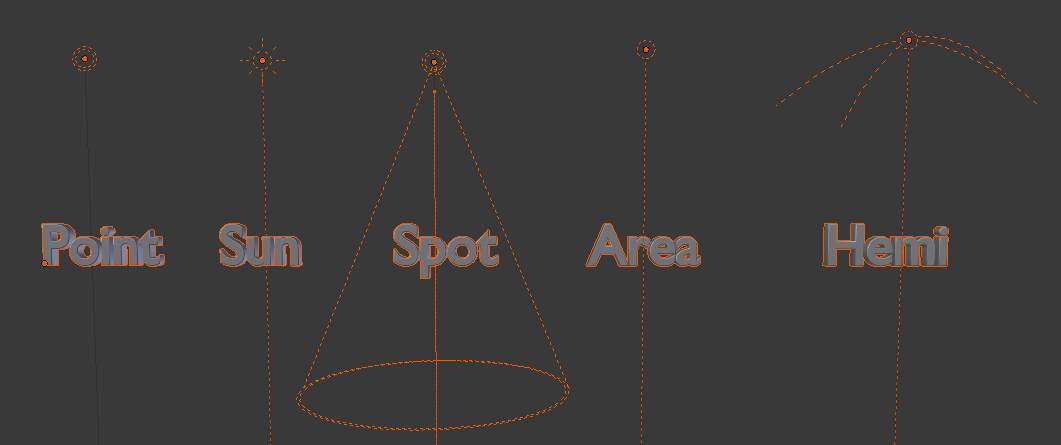
\includegraphics[scale=0.29]{lampes}
    \begin{itemize}
        \item Encore un outil indispensable car il va déterminer l'éclairage de la scène.
        \vspace{0.25cm}
        \item Voici une même scène sous les différents éclairages :
    \end{itemize}
    \vspace{5cm} 
    \begin{itemize}
        \item \textbf{Point}
        \item Éclaire comme une ampoule
        \vspace{1cm}
        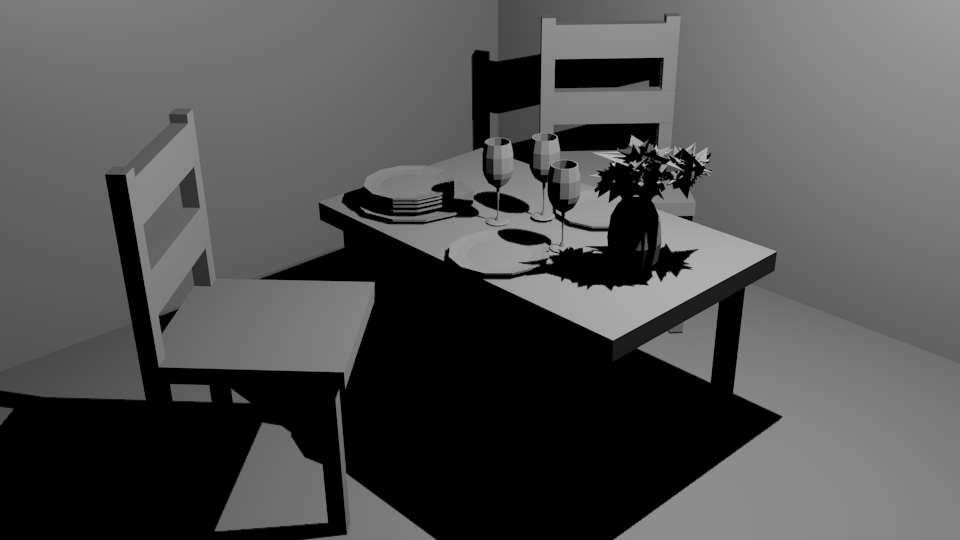
\includegraphics[scale=0.24]{point}
        \vspace{1cm}
        \item \textbf{Sun}
        \item Éclaire glogalement la scène, seule son orientation compte
        \item Sa luminosité est également plus élevée
        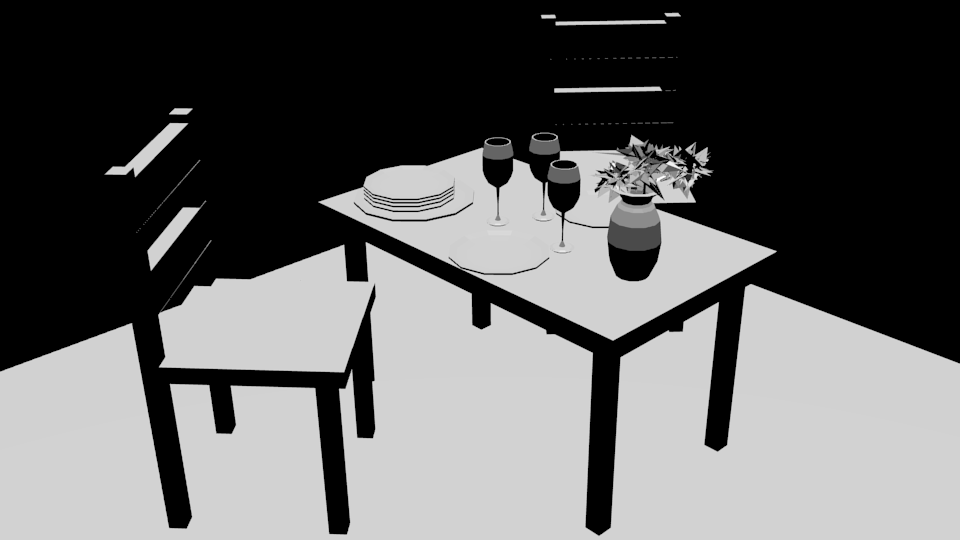
\includegraphics[scale=0.24]{sun}
        \vspace{1cm}
        \item \textbf{Spot}
        \item Éclaire en cône vers un endroit bien précis
        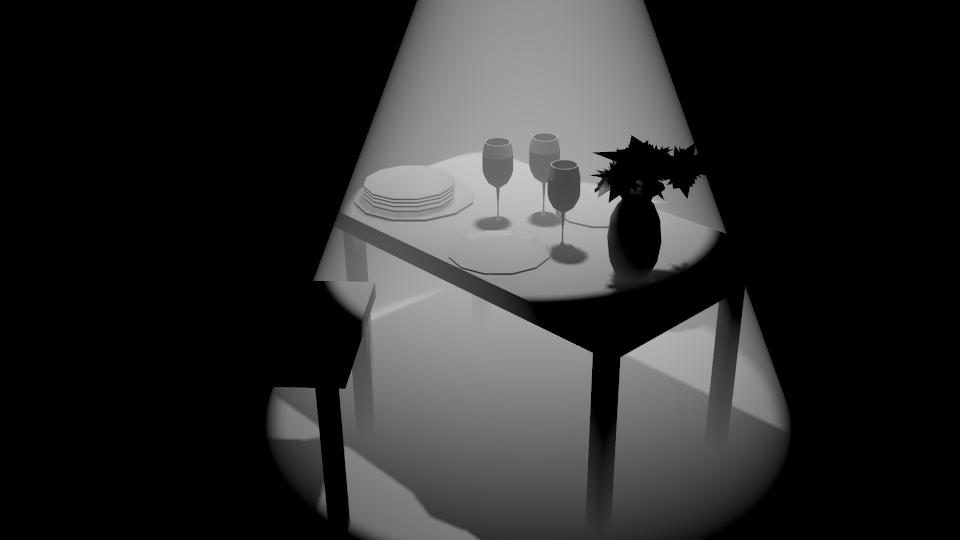
\includegraphics[scale=0.24]{spot}
        \vspace{2cm}
        \item \textbf{Area}
        \item Même éclairage que le spot mais à partir d'une surface
        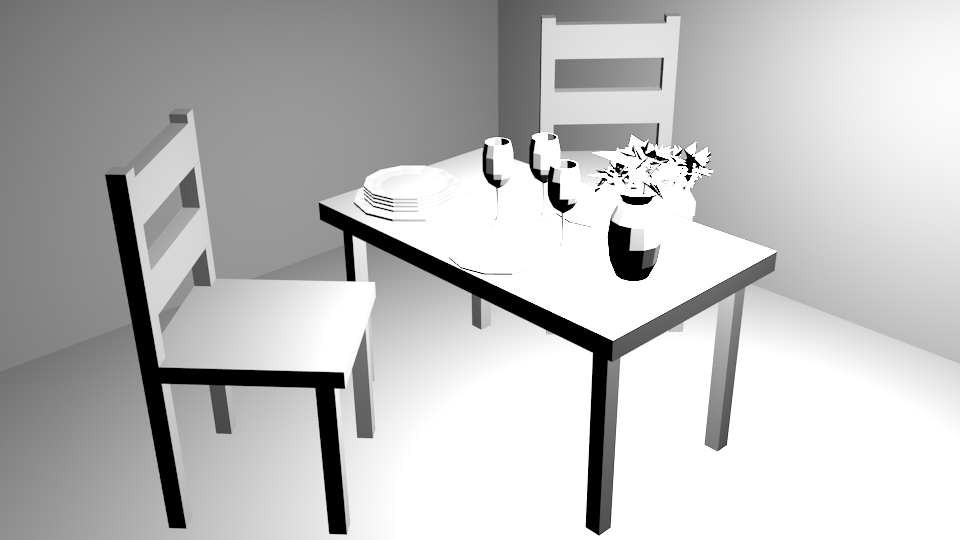
\includegraphics[scale=0.24]{area}
        \vspace{2cm}
        \item \textbf{Hemi}
        \item Éclaire comme un dôme de lumière
        \item Ne crée pas d'ombre
        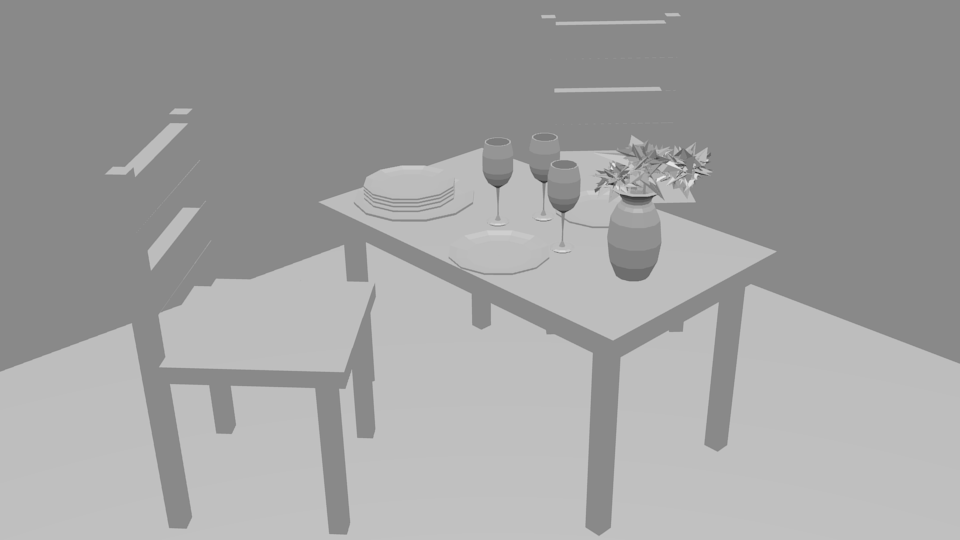
\includegraphics[scale=0.24]{hemi}
    \end{itemize}
\end{frame}

%%%%%%%%%%%%%%%%%%%%%%%%%%%%%%%%%%%%%%%%%%%%%%%%%%
\subsection{Textures}
\begin{frame}{Textures}
\begin{itemize}
    \item \textbf{Principe :} Donner du réalisme aux objets, pour cela il existe deux types de textures
    \begin{itemize}
        \item \textit{Texture Procédurale :} générée à partir d'un algorithme (et donc modifiable)
        \item \textit{Texture Image :} fichier externe à Blender qu'il va falloir charger dans le logiciel avant de pouvoir l'utiliser
    \end{itemize}
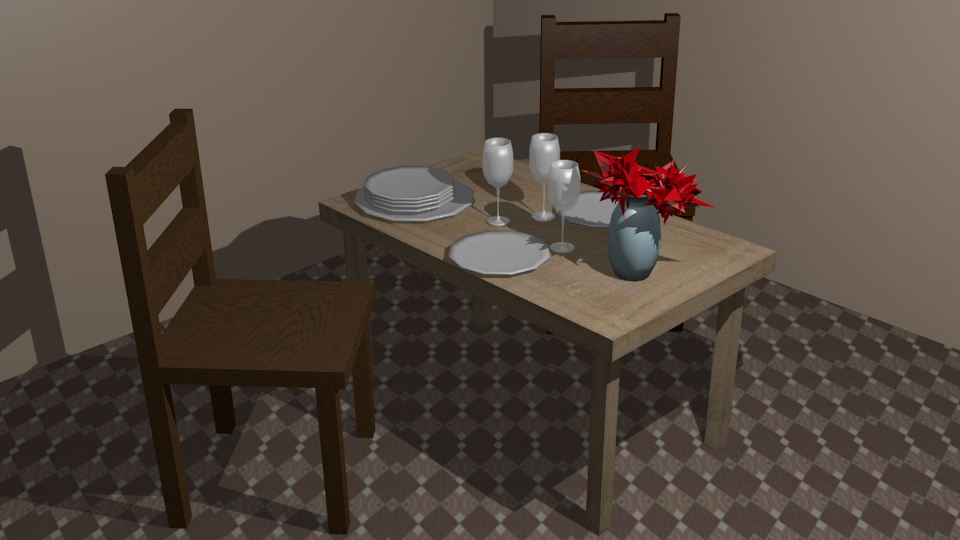
\includegraphics[scale=0.24]{tabletex}
\end{itemize}
\end{frame}
%%%%%%%%%%%%%%%%%%%%%%%%%%%%%%%%%%%%%%%%%%%%%%%%%%
\section{\scshape Animation}
\begin{frame}[c]{}
    \centering
    \huge
    \textbf{Animation}
\end{frame}

%%%%%%%%%%%%%%%%%%%%%%%%%%%%%%%%%%%%%%%%%%%%%%%%%%
\subsection{Ikey et IPO curves}
\begin{frame}{Animation}
    \begin{itemize}
        \item Blender dispose de son propre moteur de jeu \textit{Blender Game Engine} qui lui permet de réaliser des animations
        \item Quelques outils clefs :
        \begin{itemize}
            \item Ikey
            \item IPO curves
            \item Tracking
            \item Armature
        \end{itemize}
    \end{itemize}
\end{frame}

%%%%%%%%%%%%%%%%%%%%%%%%%%%%%%%%%%%%%%%%%%%%%%%%%%
\begin{frame}{Ikey}
\begin{itemize}
    \item \textit{Ikey} pour \textbf{I}nsert \textbf{Key}
    \item \textbf{Principe :} Sauvegarder certains paramètres d'un objet à un temps donné \par
        Blender se chargera d'effectuer une évolution progressive de l'objet entre deux Ikey
    \item \textit{démo}
\end{itemize}
\end{frame}

%%%%%%%%%%%%%%%%%%%%%%%%%%%%%%%%%%%%%%%%%%%%%%%%%%
\begin{frame}{IPO curves}
\begin{itemize}
    \item \textit{IPO} pour \textbf{I}nter\textbf{PO}lation et \textit{curves} pour \textbf{courbes}
    \item Ce sont les courbes générées par Blender et qui représentent le déplacement de l'objet \par
    Il est possible de les modifier directement depuis la fenêtre \textit{Graph Editor}
    \item \textit{démo}
\end{itemize}
\end{frame}

%%%%%%%%%%%%%%%%%%%%%%%%%%%%%%%%%%%%%%%%%%%%%%%%%%
\subsection{Track to}
\begin{frame}{Track to}
\begin{itemize}
    \item \textbf{Principe :} lier la caméra à un objet dont elle suivra les déplacements
    \item Le principal avantage est de ne plus avoir à régler manuellement le cadrage de la caméra pour suivre les déplacements de l'objet
    \item \textit{démo}
\end{itemize}
\end{frame}
%%%%%%%%%%%%%%%%%%%%%%%%%%%%%%%%%%%%%%%%%%%%%%%%%%

\subsection{Armature}
\begin{frame}{Armature}
    \begin{itemize}
        \item Blender permet de créer un objet appelé \textit{Single Bone}
        \item En l'extrudant, on peut créer un squelette/une armature entière qui permettra d'animer plus simplement un ensemble de meshes (un personnage par exemple)
        \item \textit{démo}
    \end{itemize}
\end{frame}

%%%%%%%%%%%%%%%%%%%%%%%%%%%%%%%%%%%%%%%%%%%%%%%%%%
\section{\scshape Utilisations par des professionnels}
\begin{frame}[c]{}
    \centering
    \huge
    \textbf{Utilisations professionnelles}
\end{frame}

%%%%%%%%%%%%%%%%%%%%%%%%%%%%%%%%%%%%%%%%%%%%%%%%%%
\subsection{Blender et Python}
\begin{frame}{Blender et Python}
    \begin{itemize}
        \item Blender dispose d'une API Python\\
        \item Une API (pour \textit{Application Programming Interface}) est comme un "mode d'emploi" qui permettrait à un système informatique d'utiliser les fonctionnalités d'un autre système informatique
        \item C'est une alternative à l'interface graphique (GUI \textit{Graphical User Interface})
    \end{itemize}
\end{frame}


%%%%%%%%%%%%%%%%%%%%%%%%%%%%%%%%%%%%%%%%%%%%%%%%%%
\subsection{Exemples}
\begin{frame}[fragile, allowframebreaks]{Utilisation pour créer une image}
    \begin{itemize}
        \item Old Guy par Kamil\\
    \end{itemize}
    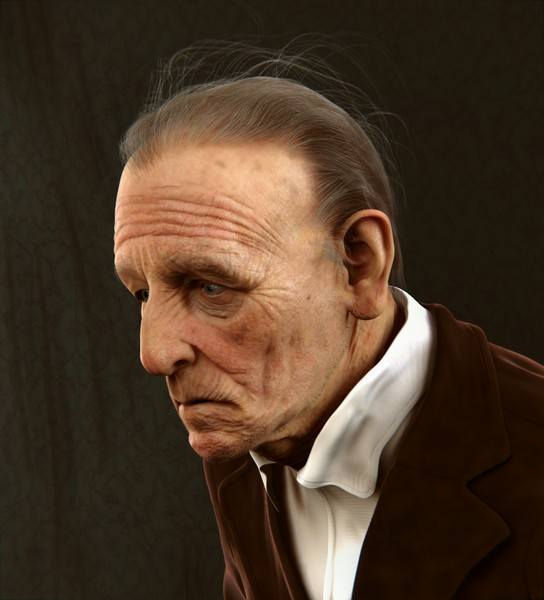
\includegraphics[scale=0.29]{oldman}
    \item Cl Hall par Yaroslav Lebidko\\
    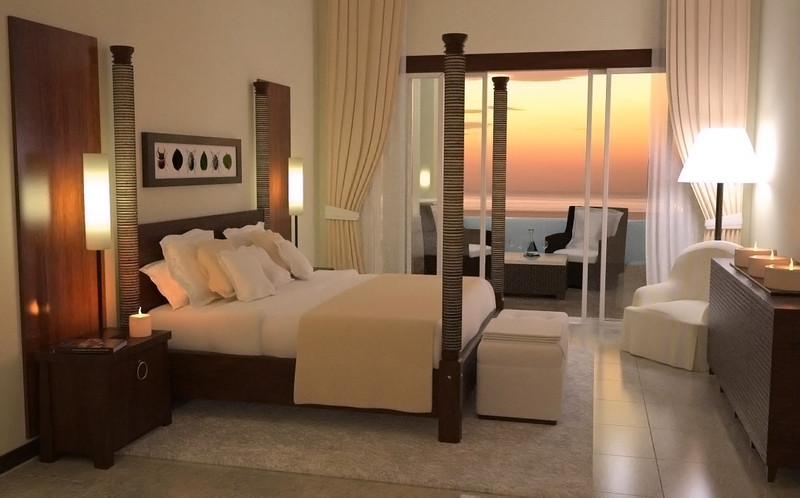
\includegraphics[scale=0.30]{chambre}\\
    \textit{http://archive.blender.org/features-gallery/gallery/}\\
\end{frame}

%%%%%%%%%%%%%%%%%%%%%%%%%%%%%%%%%%%%%%%%%%%%%%%%%%
\begin{frame}{Utilisation de Blender dans un jeu vidéo}
    \begin{itemize}
        \item Yo Frankie!\\
    \end{itemize}
    \textit{https://apricot.blender.org/}\\
    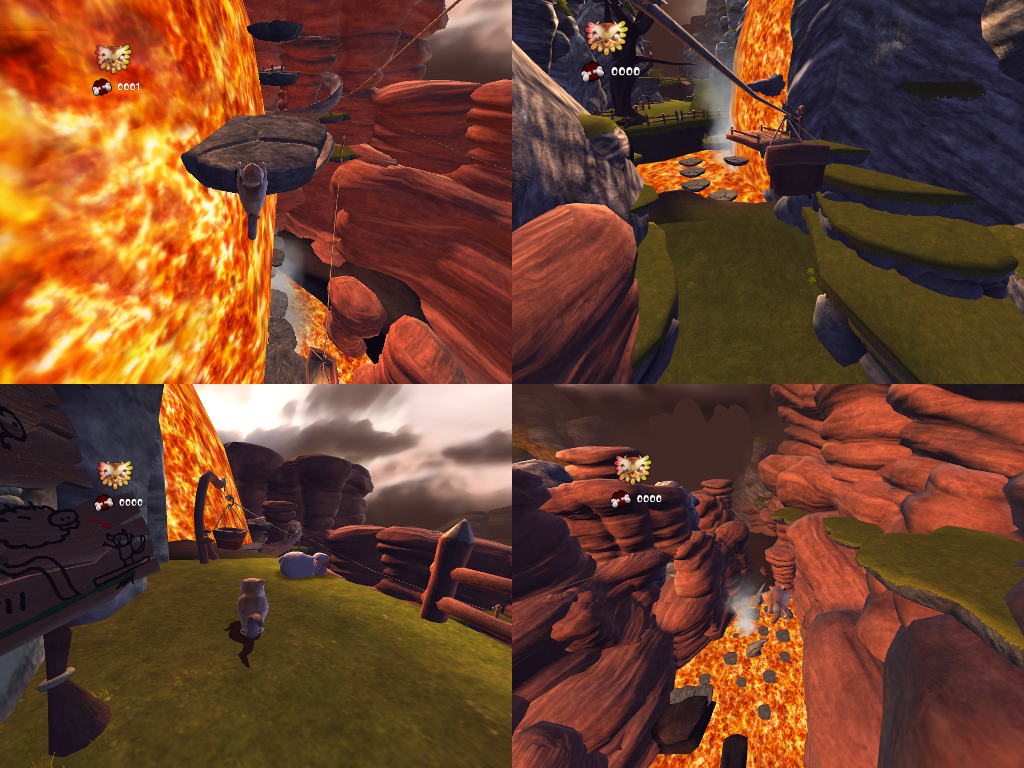
\includegraphics[scale=0.35]{frankie}
\end{frame}

%%%%%%%%%%%%%%%%%%%%%%%%%%%%%%%%%%%%%%%%%%%%%%%%%%
\begin{frame}{Exemple de vidéo réalisée avec Blender}
    \begin{itemize}
        \item Caminandes 3\\
        \textit{https://www.youtube.com/watch?v=6U1bsPCLLEg}
    \end{itemize}
\end{frame}

%%%%%%%%%%%%%%%%%%%%%%%%%%%%%%%%%%%%%%%%%%%%%%%%%%
\section{\scshape Conclusion}
\begin{frame}{Conclusion}
    \begin{itemize}
        \item Blender est un logiciel gratuit qui a l'avantage de tenir la comparaison face à d'autres logiciels d'animation payants (3D Studio max, Cinema 4D, Maya)\\
        \item Un de ses points faibles était son interface graphique difficile à appréhender mais depuis son passage à l'Open Source, elle est beaucoup plus accessible
        \item De plus, sa complexité est justifiée par les possibilités de modélisation presque infinies offertes par Blender
    \end{itemize}
\end{frame}

\end{document}